%% -*- coding:utf-8 -*-

\settowidth\jamwidth{(\ili{Deutsch})}

\chapter{Phänomene}

Dieses Kapitel befasst sich mit der Variation in den germanischen\il{Germanisch} Sprachen in dem Bereich, der oft als Kerngrammatik
bezeichnet wird, das heißt mit Sätzen vom Typ \emph{Karl liebt Maria}.\footnote{%
  \citet[\page 7--8]{Chomsky81a} schlägt vor, Grammatiken natürlicher Sprachen in einen "`Kern"' und eine "`Peripherie"' zu unterteilen.
Alle regelmäßigen Teile gehören zum Kern. Die Kerngrammatik einer Sprache wird als eine Instanz der
Universalgrammatik (UG) angesehen, der genetisch determinierten angeborenen Sprachfähigkeit des Menschen. Idiome
und andere unregelmäßige Teile einer Sprache gehören zur Peripherie. Dieses Buch befasst sich mit Phänomenen,
die üblicherweise als Teil des Kerns angesehen werden, ohne diese Kern/Peripherie-Unterscheidung anzunehmen und ohne
eine UG anzunehmen \citep{MuellerKernigkeit,MuellerCoreGram}.
} Wir werden uns Unterschiede in
der Verbstellung (Verb vor Objekt und Objekt vor Verb) ansehen, die Verbzweiteigenschaft, die
alle germanischen\il{Germanisch} Sprachen mit Ausnahme des \ili{Englisch}en haben, die Abfolge von Subjekten und
Objekten zueinander, die Stellung von Adverbialen, die Existenz/Nichtexistenz von
Verbalkomplexen, die Obligatheit/Abwesenheit von Subjekten, das Passiv einschließlich des persönlichen und
unpersönlichen Passivs, Expletivpronomen und verschiedene Möglichkeiten, den \isi{Satztyp} zu markieren, das heißt
zu signalisieren, ob ein bestimmter Satz eine Aussage, eine Frage oder ein eingebetteter Satz ist.

In diesem Kapitel werden die Phänomene vorgestellt, die dann in den
Kapiteln~\ref{chap-valence}--\ref{chap-expletives} detaillierter besprochen und analysiert werden.

Ein Wort der Vorsicht ist hier nötig: Insbesondere die folgenden drei Unterabschnitte sind potenziell
verwirrend. Eine Sprache wie das \ili{Deutsch}e wird als Subjekt-Objekt-Verb-Sprache, als Verbzweitsprache und
als Sprache mit freier Konstituentenabfolge klassifiziert \citep{Haftka96a}. Das klingt widersprüchlich, ist es aber nicht. Die jeweiligen
Klassifikationen beziehen sich auf Eigenschaften von Sprachen, nicht auf die Form einzelner Sätze.

\section{Abfolge von Subjekt, Objekt und Verb}
\label{sec-intro-svo}

Die\is{Abfolge|(}\is{Abfolge!SVO|(}\is{Abfolge!SOV|(} Sprachen der Welt können nach der jeweils
dominanten Abfolge von Subjekt, Objekt und Verb klassifiziert werden \citep{Greenberg63a-u}. Um Sprachen vergleichbar zu machen, wird für eine solche Klassifikation eine sehr allgemeine Definition grammatischer
Funktionen wie Subjekt und Objekt verwendet.
Die Definition basiert auf semantischen Eigenschaften: Subjekte sind diejenigen
Argumente, die agensartig sind, und Objekte sind Argumente, die eher patiensartig sind. Diese Definition
ist nicht immer identisch mit den einzelsprachlichen Definitionen. Zum Beispiel bezieht sich die
einzelsprachliche Definition des Subjekts im \ili{Deutsch}en (und in den germanischen\il{Germanisch} Sprachen im Allgemeinen)
auf Eigenschaften wie den Nominativ\is{Kasus!Nominativ} \citep{Reis82}, Subjekt-Verb-\isi{Kongruenz} und Kontrolle. Wir werden uns damit in
Abschnitt~\ref{sec-subj-properties} genauer befassen. Nach er Definition von Reis ist die Phrase \emph{der
  Aufsatz} in (\mex{1}) das Subjekt, obwohl sie unbelebt und kein Agens ist:
\ea
Der Aufsatz interessiert mich.
\z

\noindent
Abbildung~\vref{fig-sov-wals} zeigt die dominante Abfolge von Subjekt, Objekt und Verb in den Sprachen der Welt.
Nach \citet{Dryer2013a} ist die dominante Abfolge wie folgt definiert:

%Dominante Abfolge (Dryer: Determining Dominant Word Order):
%\largerpage
\begin{quote}
Where a language is shown on one of the word order maps as having a particular order as the dominant
order in the language, this means that it is either the only order possible or the order
that is more frequently used. \citep{Dryer2013a}
\end{quote}
%
%% I base my classification of Macushi here on the frequency counts, and since no order is more than
%% twice as frequent as the next most frequent order, I treat this language as lacking a dominant order
%% of subject, object, and verb.
%
%% Deutsch, Niederländisch und Friesisch sind V2-Sprachen, that is die SVO- und SVAuxOV-Stellungen kommen
%% durch die Voranstellung des Verbs zustande, die eine Funktion hat. Wir zählen diese Sprachen also
%% mit zu den SOV-Sprachen.
%
\begin{figure}
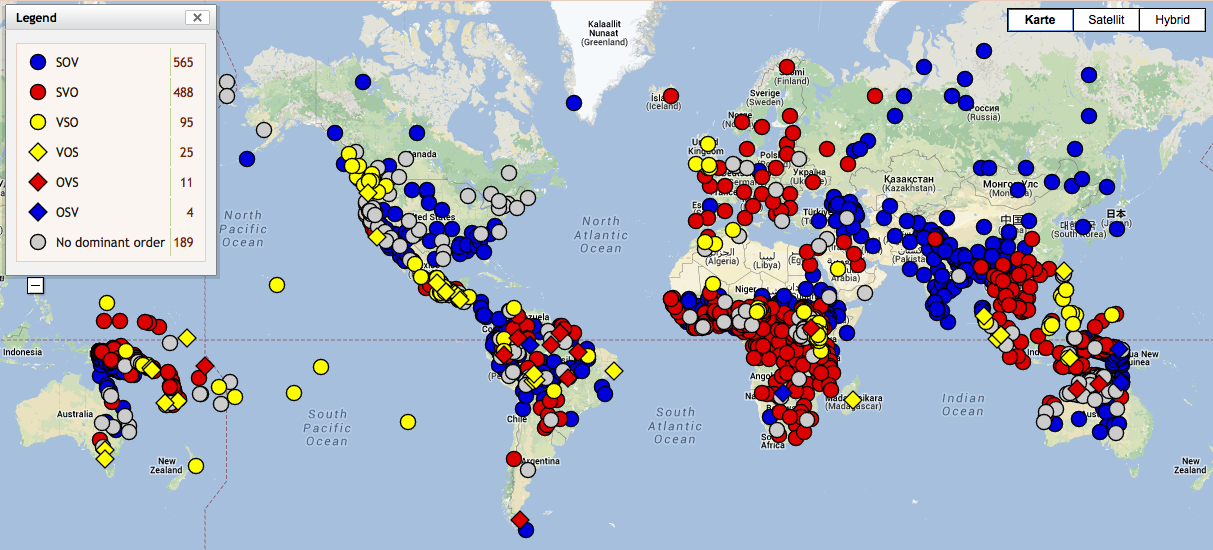
\includegraphics[width=\textwidth]{Pictures/WALS-SOV}
\caption{\label{fig-sov-wals}\citet[Abschnitt~1]{Dryer2013c}: Feature 81A: Order of subject, object and verb, The World Atlas of Language Structures}
\end{figure}

Wenn wir hineinzoomen, um die europäischen Sprachen anzuzeigen, erhalten wir Abbildung~\vref{fig-sov-wals-europe}.
\begin{figure}
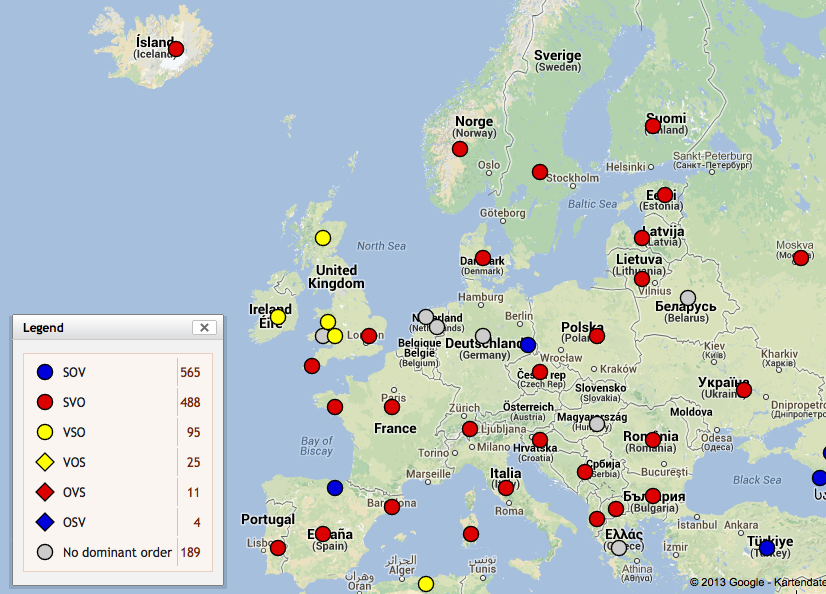
\includegraphics[width=.898\textwidth]{Pictures/WALS-SOV-Europa}
\caption{\label{fig-sov-wals-europe}Dominante Abfolgen von Subjekt, Objekt und Verb in Europa}
\end{figure}
Nach dem WALS sind \ili{Isländisch}, \ili{Norwegisch}, \ili{Schwedisch}, \ili{Dänisch} und \ili{Englisch} SVO-Sprachen.
\ili{Niederländisch}, \ili{Deutsch} und \ili{Friesisch} hingegen sind grau markiert, das heißt, diese Sprachen wurden
als Sprachen ohne dominante Abfolge eingeordnet.\footnote{
  \citet[\page 87]{Greenberg63a-u} führte das \ili{Deutsch}e und das \ili{Niederländisch}e unter den SVO-Sprachen auf.%
} Nach Abbildung~\vref{fig-sov-wals-europe-two} haben diese Sprachen
zwei dominante Abfolgen, nämlich SOV und SVO.
\begin{figure}
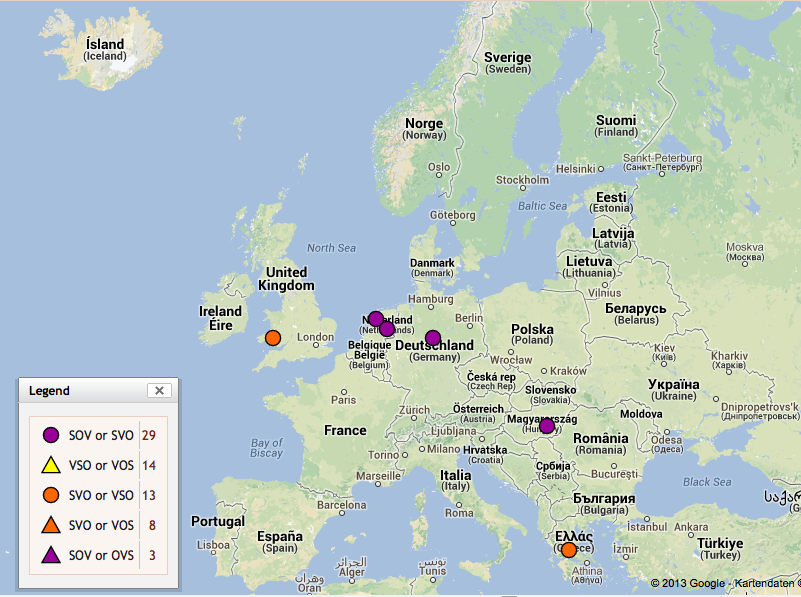
\includegraphics[width=.898\textwidth]{Pictures/WALS-SOV-Europa-no-dominant}
\caption{\label{fig-sov-wals-europe-two}%Dryer: Feature 81b:
Zwei dominante Abfolgen von Subjekt, Objekt und Verb \citep[Abschnitt~3]{Dryer2013c}}
\end{figure}
%% https://wals.info/chapter/81
%% A third subtype of language lacking a dominant order consists of languages in which different word orders occur but the choice is syntactically determined. For example, in \ili{German} and \ili{Dutch}, the dominant order is SVO in main clauses lacking an auxiliary and SOV in subordinate clauses and clauses containing an auxiliary (see below for examples). Because this results in both orders being common, neither order is considered dominant here and these two languages are shown on the map as lacking a dominant word order. In general, if the word order varies according to whether there is an auxiliary verb, the language is shown on the map as lacking a dominant order. Another language whose word order depends both on whether there is an auxigermliary and whether the clause is a main clause is Dinka (Nilotic; Sudan): like \ili{German}, the order is SVO in main clauses without an auxiliary, SAuxOV in main clauses with an auxiliary, but it is VSO in subordinate clauses without an auxiliary and AuxSOV in subordinate clauses with an auxiliary (Nebel 1948: 9, 25, 42, 75, 82).
Der Grund für diese Klassifikation ist, dass \citet[Abschnitt~1]{Dryer2013c} zwischen Sätzen unterscheidet, in denen das finite
Verb das Hauptverb ist (\mex{1}a), und Sätzen, in denen das finite Verb ein Hilfsverb ist wie in (\mex{1}b):
%\largerpage
\eal
\ex
Kim sieht den Fuchs.
\ex
Kim hat den Fuchs gesehen.
\zl
Nach Dryer ist das Muster für (\mex{0}a) SVO und das für (\mex{0}b) SAuxOV, wobei Aux
für Hilfsverb (auxiliary verb) steht. Wie
\citet{Greenberg63a-u}\footnote{%
  Siehe \citew[\page 20--21]{HoehleTopo}.
} zählt Dryer das letztere Muster zur SOV-Abfolge. Die Frage ist, ob man Hilfsverben
bei der Untersuchung der Konstituentenabfolge ignorieren kann. Das Hilfsverb \emph{hat} in (\mex{0}b) verhält sich syntaktisch
wie das Vollverb \emph{scheint} in (\mex{1}):
\ea
Kim scheint den Fuchs zu sehen.
\z
Hier hätten wir also eine SVOV-Abfolge, etwas, das in der diskutierten Typologie nicht existiert.
Die in Abbildung~\ref{fig-sov-wals-europe-two} als nicht über eine dominante Abfolge verfügend markierten Sprachen verwenden die
Verbstellung, um den Satztyp zu markieren: Es ist nur das finite Verb, das in der ersten oder zweiten
Position steht. Nichtfinite Verben stehen final:
\ea
Kim scheint den Fuchs gesehen zu haben.
\z
In Nebensätzen erscheinen sowohl das finite Verb als auch die infiniten Verben in Endstellung, während
das finite Verb in Fragen und deklarativen Hauptsätzen in Initialstellung\footnote{%
  Ich verwende den Begriff Initialstellung, um die Position zu bezeichnen, die das finite Verb in V1- oder V2-Sätzen hat. Die
  Analyse von V2 und V1 beinhaltet die Voranstellung des finiten Verbs. In V2-Sätzen wird zusätzlich
  eine Konstituente vorangestellt.
} steht.
Eine Klassifikation, die ausschließlich auf dem Zählen von Mustern beruht, ohne Hilfsverben und die
Unterscheidung zwischen Finitheit und Nichtfinitheit zu berücksichtigen, kann man diese Stellungstypen nicht auseinanderhalten \citep[Abschnitt~3]{HoehleTopo}. Im Folgenden werden wir uns Haupt- und Nebensätze mit
sowohl finiten als auch infiniten Verben ansehen. Nebensätze offenbaren Unterschiede zwischen OV- und VO-Sprachen, und ich werde argumentieren, dass das \ili{Afrikaans}, das \ili{Niederländisch}e,
das \ili{Deutsch}e und das \ili{Friesisch}e zu den OV-Sprachen gezählt werden sollten und dass das andere beobachtbare Muster
SVO auf andere Eigenschaften dieser Sprachen zurückzuführen ist, nämlich darauf, dass sie den Satztyp durch die Verbstellung
markieren und dass sie Verbzweitsprachen (V2-Sprachen) sind.\footnote{%
  Die Eigenschaft, eine V2-Sprache zu sein, ist unabhängig von der SVO/SOV-Unterscheidung. Alle germanischen\il{Germanisch}
  Sprachen außer dem \ili{Englisch}en sind V2-Sprachen. Siehe Abschnitt~\ref{sec-phenomenon-v2} zu V2.
}

Wenn man komplexere deutsche\il{Deutsch} Sätze mit mehreren Verben bildet, wird das einbettende Verb üblicherweise
rechts von den eingebetteten Verben realisiert.
%\itdopt{M: Are these notions defined somewhere?}
% Yes, in the text immediately following.
Das wird in (\mex{1}) gezeigt. (\mex{1}a) zeigt einen einfachen
Satz mit einem finiten Verb. Wenn wir das Perfekt wie in (\mex{1}b) bilden, muss das Perfekthilfsverb
dem Partizip folgen. Das Hilfsverb ist das finite Verb und es bestimmt die Form des
Partizips. Daher ist das finite Verb das Verb, das das Partizip einbettet. Das wird durch die
niedrigere Nummer von \emph{hat} im Vergleich zu \emph{gesehen} angezeigt. Wenn wir einen noch komplexeren
Satz bilden, indem wir ein weiteres Verb hinzufügen, wird dieses Verb rechts von den vorhandenen Verben angeordnet
(\mex{1}c).  Das dänische\il{Dänisch} Beispiel in (\mex{2}c), das ich leicht angepasst von \citet[\page
146]{Oersnes2009b} übernommen habe, entspricht dem deutschen\il{Deutsch} Beispiel in (\mex{1}c).

\eal
\ex
dass sie ihn sieht$_1$\german
\ex
dass sie ihn gesehen$_2$ hat$_1$
\ex
dass sie ihn gesehen$_3$ haben$_2$ muss$_1$
\zl
\eal
\label{ex-Danish-embedding}
\ex
\gll at   hun ser$_1$ ham\\
     dass sie  sieht    ihn\\\jambox{(\ili{Dänisch})}
\glt `dass sie ihn sieht'
\ex
\gll at   hun have$_1$ set$_2$ ham\\
     dass sie  hat      gesehen ihn\\
\glt `dass sie ihn gesehen hat'
\ex
\gll at   hun må$_1$ have$_2$ set$_3$ ham\\
     dass sie  muss   haben    gesehen ihn\\
\glt `dass sie ihn gesehen haben muss'
\zl
%
Wie die Beispiele in (\mex{0}) zeigen, werden die Verben im \ili{Dänisch}en vor den eingebetteten
Verben hinzugefügt. Das ist auch im \ili{Englisch}en der Fall, das hier zum Dänischen völlig
parallel wäre. Im \ili{Dänisch}en und \ili{Englisch}en gehen die
Verben dem Objekt (\emph{ham}/\emph{him}) voran, und im \ili{Deutsch}en folgen sie ihm
(\emph{ihn}).\footnote{
In deutschen\il{Deutsch} Dialekten gibt es viel Variation, was die Abfolge der Verben angeht, und sogar
das Standarddeutsche\il{Deutsch} erlaubt Abfolgen, in denen einbettende Verben den eingebetteten Verben vorangehen \parencites[\page 63--64]{Bech55a}[\page 180]{dBE83a}:
\ea
weil er nicht wird$_1$ haben$_2$ kommen$_4$ können$_3$
\z
Die Abfolge, in der das einbettende Verb dem eingebetteten Verb vorangeht, ist im \ili{Niederländisch}en Standard \citep[\page 159]{dBE83a}. Kapitel~\ref{chap-verbal-complex}
bietet eine Analyse des Verbalkomplexes in den germanischen\il{Germanisch} OV-Sprachen. Die Verbalkomplexe folgen immer den Objekten.
}

\textcites[\page 15]{Haider2010a}[Abschnitt~15.2]{Haider2020a} weist auf zwei weitere Unterschiede zwischen den germanischen\il{Germanisch} VO- und OV-Sprachen hin:
Partikeln gehen Verben in OV-Sprachen voran \citep[Abschnitt~2.4]{Vikner2001a}, und dasselbe gilt für resultative sekundäre
Prädikate. In VO-Sprachen folgen Partikeln und Resultatprädikate dem Verb. Das wird durch
die folgenden zwei Beispielsätze demonstriert:
%\itdopt{AZ: Kim will look the information up is also possible, footnote?}
\eal
\ex Kim will look up the information.
\ex
Kim wird die Information nachschlagen.\german
\zl
\eal
\ex Kim will fish the pond empty.
\ex
Kim wird den Teich leer fischen.\german
\zl
(\mex{-1}a) zeigt, dass \emph{look} der Partikel \emph{up} vorangeht, während das Verb \emph{schlagen}
im \ili{Deutsch}en der Partikel \emph{nach} folgen muss. Ebenso folgt das sekundäre resultative
Prädikat \emph{empty} dem Verb in (\mex{0}a), aber \emph{leer} geht dem Verb in
(\mex{0}b) voran. Man beachte, dass ich in den Beispielen ein Futurhilfsverb verwendet habe, um Nebeneffekte zu vermeiden, die
auf die Verbzweiteigenschaft des \ili{Deutsch}en zurückzuführen sind: In deklarativen Hauptsätzen geht das finite Verb immer
Partikeln und Resultatprädikaten voran, aber das ist auf den Satztyp zurückzuführen (siehe Abschnitt~\ref{sec-phenomenon-v2}).

%\largerpage[-2]
Ich werde in Kapitel~\ref{chap-verb-position} auf die SVO- vs.\ SOV-Abfolge zurückkommen und mehr von der
Evidenz liefern, die in der Literatur verwendet wurde, um für den OV-Status von Sprachen wie dem \ili{Deutsch}en und dem \ili{Niederländisch}en zu argumentieren.
%\itdopt{M: descriptive OV status is compatible with comparative VO/OV classification.}

Während die germanischen\il{Germanisch} Sprachen sich gut in SOV-Sprachen mit Scrambling (siehe
Abschnitt~\ref{sec-phenomenon-scrambling} weiter unten) und SVO-Sprachen ohne Scrambling aufteilen lassen, gibt es eine
Ausnahme: das \ili{Jiddisch}e. Die folgenden Daten aus \begin{NoHyper}\citew[\page 402]{Diesing97a}\end{NoHyper} zeigen, dass das \ili{Jiddisch}e
die Abfolge haben kann, die üblicherweise in SVO-Sprachen beobachtet wird (\mex{1}a), und die Abfolgen, die in SOV-Sprachen
mit Scrambling beobachtet werden (\mex{1}b, c). Es kann aber auch die Abfolgen in (\mex{1}d) und
(\mex{1}e) haben, in denen das Verb in der Mitte steht und entweder das direkte Objekt oder das indirekte Objekt
dem Verb vorangeht.

\eal
\label{ex-yiddish-vo-ov}
\ex
\gll Maks hot nit gegebn Rifken dos bukh.\\
     Max  hat nicht gegeben  Rifken das Buch\\\yiddish
\glt `Max hat Rifken das Buch nicht gegeben.'
\ex
\gll Maks hot Rifken dos bukh nit gegebn.\\
     Max  hat Rifken das Buch nicht gegeben\\
\glt `Max hat Rifken das Buch nicht gegeben.'
\ex
\gll Maks hot dos bukh Rifken nit gegebn.\\
     Max  hat das Buch Rifken nicht gegeben\\
\glt `Max hat Rifken das Buch nicht gegeben.'
\ex
\gll Maks hot Rifken nit gegebn dos bukh.\\
     Max  hat Rifken nicht gegeben  das Buch\\
\glt `Max hat Rifken das Buch nicht gegeben.'
\ex
\glt Max hat dos bukh nit gegebn Rifken.\\
     Max hat das Buch nicht gegeben  Rifken\\
\glt `Max hat Rifken das Buch nicht gegeben.'
\zl
Es wurde behauptet, das \ili{Jiddisch}e sei eine VO-Sprache
\parencites[\page 113]{dBMvW86a}[\page 388]{Diesing97a}{Sadock98a} oder eine OV-Sprache
\parencites{Hall79a}{Geilfuss90a-u}[Kapitel~2]{Vikner2001a}. Einige Forscher haben argumentiert, dass es
keines von beiden sei: Es wäre ein dritter Sprachtyp, einer mit gemischtem VO/OV-Status \parencites{Santorini93a}[\page 12]{Schallert2007a}[\page 161]{Haider2010a}{Haider2020a}.

%%\largerpage[2]
\citet[Abschnitt~2.5]{Schallert2007a} weist darauf hin, dass viele germanische\il{Germanisch} Sprachen früherer Stufen keine
feste VO- oder OV-Abfolge hatten, und ordnet sie zusammen mit dem \ili{Jiddisch}en dieser dritten Klasse von Sprachen mit
eher freier Verbstellung zu. Seine Klassifikation ist in Tabelle~\ref{table-VO-OV} angegeben.
 
\begin{table}
\oneline{%
\begin{tabular}{llll}\lsptoprule
               & OV-Sprachen                   & VO-Sprachen                   & OV/VO-Sprachen\\\midrule
Nordgermanisch\il{Germanisch} &                                & \ili{Isländisch}, \ili{Färöisch}, & Altnordisch\il{Nordisch!Alt-}, \\
               &                                & \ili{Norwegisch}, \ili{Dänisch}, & (Altisländisch\il{Isländisch!Alt-})\\
               &                                & \ili{Schwedisch}                  &\\
Westgermanisch\il{Germanisch}  & \ili{Deutsch}, \ili{Niederländisch},     & \ili{Englisch}                  & \ili{Jiddisch}, Altenglisch\il{Englisch!Alt-}, \\
               & \ili{Afrikaans}, \ili{Friesisch} &                                & Althochdeutsch\il{Deutsch!Althoch-}, \\
\lspbottomrule
\end{tabular}}
\caption{Konstituentenabfolge-Typologie der germanischen Sprachen nach \citet[\page 13]{Schallert2007a}}\label{table-VO-OV}
\end{table}
\is{Abfolge|)}\is{Abfolge!SVO|)}\is{Abfolge!SOV|)}

\section{V2}
\label{sec-phenomenon-v2}

Die\is{V2-Sprache|(}\is{Abfolge!V2|(} germanischen\il{Germanisch} Sprachen sind, mit Ausnahme des \ili{Englisch}en, sogenannte \emph{Verbzweitsprachen} (V2-Sprachen).
Die V2-Eigenschaft
lässt sich mit den folgenden deutschen\il{Deutsch} Sätzen illustrieren. (\mex{1}) zeigt deklarative Hauptsätze,
in denen eine der Konstituenten vorangestellt ist. (\mex{2}) zeigt parallele Interrogativsätze.

\eal
\ex
Das Kind gibt dem Eichhörnchen jetzt eine Nuss.\german
\ex
Dem Eichhörnchen gibt das Kind jetzt eine Nuss.
\ex
Eine Nuss gibt das Kind dem Eichhörnchen jetzt.
\ex
Jetzt gibt das Kind dem Eichhörnchen eine Nuss.
\zl
\eal
\ex
Wer gibt dem Eichhörnchen jetzt eine Nuss?\german
\ex
Wem gibt das Kind jetzt eine Nuss?
\ex
Was gibt das Kind dem Eichhörnchen jetzt?
\ex
Wann gibt das Kind dem Eichhörnchen eine Nuss?
\zl
Das finite Verb steht in allen Sätzen in (\mex{-1}) und (\mex{0}) in zweiter Position.

Das \ili{Englisch}e hingegen erlaubt keine Abfolgen, in denen das Objekt unmittelbar vor dem
finiten Verb erscheint.

\eal
\ex[*]{
This squirrel give I a nut now.
}
\ex[*]{
This nut give I a squirrel now.
}
\ex[*]{
Tomorrow give I the squirrel a nut.
}
\zl
Adverbiale und Objekte können vorangestellt werden, aber dann müssen sie vor dem Satz erscheinen, der aus
Subjekt und Verb und möglicherweise weiteren Konstituenten besteht.
\eal
\ex This nut, I give the squirrel now.
\ex Now, I give the squirrel a nut.
\zl

\noindent
Man beachte außerdem, dass die Voranstellung von Objekten bei Verben mit zwei Objekten für manche Sprecher auf das sekundäre Objekt
beschränkt ist \citep[\page 258]{Hudson92a-u}.\footnote{
  Ich verwende die Begriffe \emph{primäres Objekt}\is{Objekt!primär} und \emph{sekundäres
    Objekt}\is{Objekt!sekundär} \citep[280]{PS92a}, um die Verwirrung zu vermeiden, die manchmal
  durch die Begriffe \emph{direktes}\is{Objekt!direkt} und \emph{indirektes Objekt}\is{Objekt!indirekt} verursacht wird. Das primäre Objekt ist das erste Objekt im \ili{Englisch}en
  und das Dativobjekt von ditransitiven Verben, die den Dativ regieren, im \ili{Deutsch}en. Das sekundäre Objekt
  ist das zweite Objekt im \ili{Englisch}en und der Akkusativ in deutschen\il{Deutsch} ditransitiven Konstruktionen. Die Abfolge
  Dativ vor Akkusativ ist auch die unmarkierte Abfolge\is{Abfolge!unmarkiert} für die Argumente der meisten ditransitiven Verben
  \citep{Hoehle82a}. Zu Ausnahmen siehe \citew{Cook2006a-u}.
% \ili{Icelandic} dat primary, acc secondary
% \itdopt{M: This is very confusing because the criterion is basically semantic (recipient vs. theme)
%   whereas primary seems to suggest syntactic criteria. It's the same confusion as with
%   direct/indirect.\\
% Stefan: Yes, we are doing syntax.}
} Während also die Voranstellung des sekundären Objekts in
(\mex{1}b) von allen Sprechern erlaubt wird, finden manche Sprecher Extraktionen wie die Extraktion des
primären Objekts in (\mex{1}c) inakzeptabel oder markiert.

\eal
\judgewidth{\%}
\ex[]{
We give children sweets.
}
\ex[]{
These sweets, we give children \_.
}
\ex[\%]{
These children, we give \_ sweets.
}
\zl
In V2-Sprachen ist das nicht der Fall: Sie sind, was die Voranstellung angeht, recht
liberal. Im Prinzip können alle Konstituenten vorangestellt werden, mit Ausnahme von Reflexiv\-pronomen,
die von inhärent reflexiven Verben\is{Verb!inhärent reflexiv} selegiert werden (\mex{1}), expletiven\is{Pronomen!expletiv} Objekten (\mex{2}) und bestimmten Modal\-partikeln (\mex{3}). Siehe auch \citew[\page 159]{Hoberg81a} zu inhärent reflexiven
Verben\is{Verb!inhärent reflexiv} und Modalpartikeln.
\eal
\ex[]{
Maria erholt sich.\german
}
\ex[*]{
Sich erholt Maria.
}
\zl
\eal
\ex[]{
Er bringt es bis zum Professor.\german
}
\ex[\#]{
Es bringt er bis zum Professor.
}
\zl
\eal
\ex[]{
Er geht halt nicht.\german
}
\ex[*]{
Halt geht er nicht.
}
\zl
%\itdopt{AZ: why do you call es an EXPL in this case? it seems to be a pronominal object}
Das Element vor dem finiten Verb ist nicht notwendigerweise ein Satzgenosse des finiten Verbs. Tatsächlich
kann es zu einem tief eingebetteten Kopf gehören, wie das folgende Beispiel aus dem
\ili{Deutsch}en zeigt:
\ea
{}[Über dieses Thema]$_i$ habe ich sie gebeten, [[einen Vortrag \_$_i$~] zu halten].\footnote{
Adaptiert nach \citew[\page 21]{HN89b}.
}\german

\z
Die PP \emph{über dieses Thema} hängt von dem Nomen \emph{Vortrag} ab, das Teil der VP ist, deren Kopf
\emph{zu halten} ist. Diese VP ist unter \emph{gebeten} eingebettet. Sätze wie
(\mex{0}) zeigen, dass V2-Voranstellungen nicht als eine einfache Umstellung der Argumente eines
Verbs analysiert werden können. Während ein solcher Ansatz für die Beispiele in (\mex{1}) funktionieren würde, ließe er sich nicht auf andere
Fälle übertragen, in denen das vorangestellte Element nicht vom höchsten Verb im Satz abhängt.
\ea
Den Text kennt er.
\z

\noindent
Die folgenden Beispiele aus dem \ili{Dänisch}en (SVO) zeigen, dass die Eigenschaft, eine V2-Sprache
zu sein, unabhängig von der VO/OV-Eigenschaft ist:
\eal
\ex
\gll Gert har læst bogen.\\
     Gert hat gelesen Buch.\textsc{def}\\\danish
\glt `Gert hat das Buch gelesen.'
\ex
\gll Bogen har Gert læst.\\
     Buch.\textsc{def} hat Gert gelesen\\
\glt `Gert hat das Buch gelesen.'
\zl
Das Beispiel in (\mex{0}a) zeigt, dass das Objekt den Verben folgt, und (\mex{0}b) zeigt, dass das
Objekt \emph{bogen} in Satzanfangsstellung vor dem finiten Verb
\emph{har} erscheinen kann.

Die V2-Abfolge wird in den germanischen\il{Germanisch} Sprachen (außer dem \ili{Englisch}en) durchgängig in deklarativen Hauptsätzen verwendet.
Einige germanische\il{Germanisch} Sprachen erlauben die V2-Abfolge nicht in eingebetteten Sätzen. Für eine Diskussion
eingebetteter Interrogativsätze siehe Abschnitt~\ref{sec-embeeded-clauses}.

Während das \ili{Englisch}e die Abfolge Objekt"=Verb"=Subjekt nicht erlaubt, die in den anderen germanischen\il{Germanisch}
Sprachen aufgrund der V2-Voranstellung möglich ist, erlaubt es die Voranstellung des Objekts in Fragen, was zu
Strukturen führt, die parallel zu dem sind, was wir aus den anderen germanischen\il{Germanisch} Sprachen kennen:
\eal
\ex\label{ex-which-book-did-sandy-read}
Which book did Sandy read?
\ex\label{ex-which-book-did-sandy-give-to-kim}
Which book did Sandy give to Kim?
\ex To whom did Sandy give the book?
\zl
Das \ili{Englisch}e war früher eine V2-Sprache, hat diese Eigenschaft aber verloren. Das V2 in Fragen ist ein Überbleibsel früherer
Sprachstufen, weshalb das \ili{Englisch}e eine \emph{residuale V2-Sprache}\is{V2-Sprache!residual} genannt wird \citep[\page 375]{Rizzi1990a-u}.

V2 und Verbvoranstellung allgemein sind eine Möglichkeit, Satztypen in allen germanischen\il{Germanisch} Sprachen zu markieren. V2-Sätze
können in allen germanischen\il{Germanisch} Sprachen außer dem \ili{Englisch}en deklarative Sätze sein, und sie können in allen
germanischen\il{Germanisch} Sprachen einschließlich des \ili{Englisch}en Fragen sein. Außerdem können V2-Sätze Imperative sein, wie (\mex{1}) zeigt.
\ea
Jetzt gib ihr das Buch!
\z
Sätze mit dem finiten Verb in erster Position (V1) können Ja/Nein-Fragen oder Imperative sein:
\eal
\ex
Gibt er ihr das Buch?
\ex
Gib ihr das Buch!
\zl
Natürlich ist die Abfolge der Elemente nicht der einzige Hinweis auf den vorliegenden Satztyp. Auch Intonation und morphologische Markierung von Imperativformen spielen eine Rolle.

Die Eigenschaft, eine V2-Sprache zu sein, ist unter den Sprachen der Welt überaus selten \citep[\page
  343]{Holmberg2015a}. Abgesehen von den germanischen\il{Germanisch} Sprachen mit Ausnahme des
modernen \ili{Englisch}en \citep{HP86a-ed} sind die einzigen bekannten Fälle das \ili{Estnisch}e (Finno-Ugrisch, \citealp[\page 343]{Holmberg2015a}), das \ili{Sorbisch}e \citep[Eintrag~79]{Plank2003b-ed} (eine slawische\il{Slawisch} Sprache), die
keltischen\il{Keltisch} Sprachen \ili{Bretonisch} \citep{BK2000a-u}, \ili{Kornisch} \citep*[\page 287]{BTW2007a-u} und
Mittelwalisisch\il{Walisisch!Mittel} \citep{Willis1998a-u}, Altfranzösisch\il{Französisch!Alt-} \parencites[Abschnitt~1.3]{Adams1987a-u}[Abschnitt~2.1.2]{Roberts93a-u}[Kapitel~2]{Vance97a-u}, Altspanisch\il{Spanisch!Alt}
% Plank2003b-ed: and some other early \ili{Romance} languages
%\citep{Fontana93a,Fontana97a},
\citep[Abschnitt~3.3.2]{Fontana97a-u},
\ili{Rätoromanisch} \citep{Poletto2002a-u,Anderson2006a-u}, Kaschmiri
\citep[Kapitel~4]{Bhatt99a-u}, zwei Dialekte des \ili{Himachali}, das ebenfalls zum \ili{Indoarisch}en gehört
und in an Kaschmiri angrenzenden Regionen gesprochen wird \citep{Hendriksen90a}, die austronesischen\il{Austronesisch}
Sprachen \ili{Taiof} und \ili{Sisiqa} \citep[\page 495]{Ross2004a-u} und die brasilianische indigene
Sprache \ili{Karitiana} aus der Tupí-Sprachfamilie \citep{Storto2003a-u}.
% This is mentioned in Bayer2010, but maybe it is like the australian languages.
% and the
%Uto-Aztekian language \ili{Tohono O'odham}, which is spoken in the southwest of the US and in northern Mexico.
% Estnisch 
\is{V2-Sprache|)}\is{Abfolge!V2|)}

\section{Scrambling}
\label{sec-phenomenon-scrambling}

Während\is{Scrambling|(} die Konstituentenabfolge in Sprachen wie dem \ili{Englisch}en eher festgelegt ist, erlauben Sprachen wie das \ili{Niederländisch}e und
das \ili{Deutsch}e eine freiere Permutation der Argumente. Um die Effekte nicht durch
Umstellungen zu verfälschen, die auf die V2-Eigenschaft zurückzuführen sind, verwende ich Verbletztsätze, um das
Phänomen im \ili{Deutsch}en zu illustrieren. Beispiel (\mex{1}) zeigt die einzige mögliche Abfolge von Subjekt und Objekten eines einfachen
ditransitiven Satzes im \ili{Englisch}en ohne Extraktion:

\ea
because the child gives the squirrel the nut \english
\z
Wenn Sprecher das sekundäre Objekt \emph{the nut} vor dem primären Objekt \emph{the
  squirrel} realisieren wollen, müssen sie ein Präpositionalobjekt verwenden. Diese Art der Umstellung wird
\emph{Dative Shift} genannt, und (\mex{1}) ist ein Beispiel:
\ea
because the child gives the nut to the squirrel \english
\z
Im Gegensatz dazu haben wir die deutschen\il{Deutsch} Beispiele in (\mex{1}). Diese Beispiele zeigen, dass die Nominal\-phrasen
frei permutiert werden können:
\eal
\ex
{}[weil] das Kind dem Eichhörnchen die Nuss gibt\german
\ex
{}[weil] das Kind die Nuss dem Eichhörnchen gibt
\ex
{}[weil] die Nuss das Kind dem Eichhörnchen gibt
\ex
{}[weil] die Nuss dem Eichhörnchen das Kind gibt
\ex
{}[weil] dem Eichhörnchen das Kind die Nuss gibt
\ex
{}[weil] dem Eichhörnchen die Nuss das Kind gibt
\zl
Nicht alle dieser Abfolgen können in allen Kontexten verwendet werden. Einige der Beispiele erfordern eine besondere,
kontrastive Intonation. Die Abfolgen können nach der Anzahl der Kontexte sortiert werden, in denen
sie verwendet werden können. \citet{Hoehle82a} schlägt vor, die Abfolge, die in den meisten Kontexten verwendet werden kann, die
normale oder unmarkierte Abfolge\is{Abfolge!unmarkiert} zu nennen.

Die OV-Sprachen teilen viele Eigenschaften, sodass man erwarten würde, dass das \ili{Niederländisch}e ebenfalls Scrambling
erlaubt. Objekt-NPs können jedoch nicht gescrambelt werden:
\ea[*]{
\longexampleandlanguage{
\gll Toen hebben de  autoriteiten het kind de moeder  teruggegeven\\
     dann haben   die Behörden  das Kind die Mutter  zurückgegeben\\}{Niederländisch}
\glt Intendiert: `Die Behörden gaben das Kind der Mutter zurück.'
}
\z
Der Grund dafür ist, dass NPs im \ili{Niederländisch}en nicht kasusmarkiert sind. Es wäre für Hörer
und Leser sehr schwierig herauszufinden, wer wem was angetan hat. Das ist parallel zu Beispielen mit kasuslosen NPs im
\ili{Deutsch}en. Wie \citet[\page 45]{Wegener85b} feststellt, ist (\mex{1}) nicht mehrdeutig:
\ea
\label{ex-sie-mischt-dem-wein-wasser-bei}
Sie mischt Wein Wasser bei.
\z
Das bedeutet, dass es Wein gibt und Wasser hinzugefügt wird. Das entspricht der Abfolge dat < akk.
Die Situation ist mit Determinatoren anders:
\eal
\ex
Sie mischt dem Wein das Wasser bei.
\ex
Sie mischt das Wasser dem Wein bei.
\zl
Mit Determinatoren erhalten wir die Lesart in (\mex{-1}) unabhängig von der Abfolge der Nominalphrasen. Wenn
wir die Abfolge der determinatorlosen NPs in (\mex{-1}) ändern, erhalten wir dagegen eine andere Lesart:
\ea
Sie mischt Wasser Wein bei.
\z
Ohne jegliche Hinweise aus der Kasusmarkierung (oder dem Kontext oder der Intonation) hat man also die Abfolge dat < akk; mit
Kasusmarkierung sind beide Abfolgen möglich.
%
% Tibor 2025: Siehe etwa (ich habe das mit Simon Masloch und der wiederum mit Sarah Broll (IDS) diskutiert und das Bsp. ist von ihnen):
%
%(1) Welchem Getränk mischt Sabine Wasser bei?
%(2) Sie mischt Wasser Wein bei.
%
% in der ganzen Debatte habe ich noch vergessen, ein Beispiel nachzureichen, das unser Glossa-Papier sozusagen fortsetzt (auf das mich ebenfalls SM und SB noch aufmerksam gemacht haben):
%
% (1) Jeder weiß, dass Yoko Ono John Lennon gefällt.
%
% Hier hat man keinerlei Kasus-Markierung und dennoch kein „Freezing“ oder wie man es nennen will. Wir führen das darauf zurück, dass Beispiele mit _gefallen_ und zwei belebten Argumenten keine Abfolgepräferenzen besitzen, also in der Realisation echt optional sind (was natürlich unter der Annahme einer Basisabfolge kaum erklärbar ist).

Um auf das \ili{Niederländisch}e zurückzukommen: Die Beispiele in (\mex{1}) zeigen, dass Scrambling tatsächlich möglich ist, wenn die Argumente
identifiziert werden können \parencites[\page 989]{GHdRvdT1984a-ed}[\page 14, 152]{Haider2010a}:
\eal
\ex
\longexampleandlanguage{
\gll Toen hebben de autoriteiten het kind  aan de  moeder teruggegeven.\\
     dann haben   die Behörden das Kind  an  die Mutter zurückgegeben\\}{Niederländisch}
\glt `Dann haben die Behörden das Kind der Mutter zurückgegeben.'
\ex
\gll Toen hebben de  autoriteiten aan de moeder  het kind  teruggegeven\\
     dann haben   die Behörden  an  die Mutter  das Kind  zurückgegeben\\
\glt `Dann haben die Behörden das Kind der Mutter zurückgegeben.'
\zl
(\mex{0}) enthält Beispiele mit NP- und PP-Objekt. Da die PP klar identifizierbar ist, können die beiden
Argumente in beliebiger Abfolge erscheinen. Es scheint daher gerechtfertigt anzunehmen, dass die OV-Sprachen (das \ili{Deutsch}e,
das \ili{Niederländisch}e, das \ili{Afrikaans}, das \ili{Friesisch}e) Scrambling erlauben, mit Beschränkungen, die das Scrambling von Elementen verbieten, die
nicht identifizierbar sind.%
\is{Scrambling|)}

\section{Die Stellung von Adverbialen}
\label{sec-phenomena-position-of-adverbials}

In\is{Abfolge!Adverbiale|(} Sprachen wie dem \ili{Deutsch}en und dem \ili{Niederländisch}en ist die Stellung von Adverbialen recht frei: das Adverb \emph{gestern}
kann überall zwischen den Argumenten und dem Verb erscheinen:
\eal
\ex
weil das Kind dem Eichhörnchen die Nuss \emph{gestern} gab
\ex
weil das Kind dem Eichhörnchen \emph{gestern} die Nuss gab
\ex
weil das Kind \emph{gestern} dem Eichhörnchen die Nuss gab
\ex
weil \emph{gestern} das Kind dem Eichhörnchen die Nuss gab
\zl
Auch das \ili{Niederländisch}e hat eine freie Abfolge von Adverbialen \parencites[\page 387]{Neeleman94b-u}[\page
4]{Koster99a-u}[Abschnitt~6]{Bouma2003a-u}. (\mex{1}) zeigt die niederländischen\il{Niederländisch} Beispiele, die
(\mex{0}) entsprechen:
% Neeleman sagt, das sei base-Generation.
% Bouma2003a:6
% \eal
% \ex
% \gll dat  Kim regelmatig haar moeder bezoekt\\
%      that Kim regularly  her  mother visits\\\dutch
% \glt `that Kim visit her mother regularly'
% \ex
% \gll dat  Kim haar moeder regelmatig bezoekt\\
%      that Kim her  mother regularly  visits\\
% \glt `that Kim visit her mother regularly'
% \zl
\eal
\ex
\gll omdat het kind de eekhoorn de noot \emph{gisteren} gaf\\
     weil das Kind das Eichhörnchen die Nuss gestern gab\\\dutchshort
\glt `weil das Kind dem Eichhörnchen die Nuss gestern gab'
\ex
\gll omdat het kind de eekhoorn \emph{gisteren} de noot gaf\\
     weil das Kind das Eichhörnchen gestern die Nuss gab\\
\ex
\gll omdat het kind \emph{gisteren} de eekhoorn de noot gaf\\
     weil das Kind gestern das Eichhörnchen die Nuss gab\\
\ex
\gll omdat \emph{gisteren} het kind de eekhoorn de noot gaf\\
     weil gestern das Kind das Eichhörnchen die Nuss gab\\
\zl

\noindent
Im Gegensatz dazu ist die Stellung der Adverbiale in SVO-Sprachen wie dem \ili{Dänisch}en und dem
\ili{Englisch}en eher eingeschränkt. Die Adverbiale werden üblicherweise vor oder nach der VP platziert; das heißt, Verb und Objekte bilden eine
Einheit, und Adverbiale schließen sich links oder rechts an diese Einheit an. (\mex{1}) liefert ein Beispiel:
\eal
\ex[]{
because the child {often} [gave the squirrel the nut] \english
}
\ex[]{
because the child [gave the squirrel the nut] {often}
}
\ex[*]{
because the child [gave often the squirrel the nut]
}
\ex[*]{
because the child [gave the squirrel often the nut]
}
\zl
Es wird angenommen, dass Verb und Objekte in diesen Sprachen eine strukturelle Einheit bilden, eine Verbalphrase (VP). Adverbiale können
sich an diese VP anschließen und eine größere VP bilden, die dann mit dem Subjekt zu einem vollständigen Satz kombiniert wird.

Das folgende Beispiel, das auf \citet[§ 8.20, 495]{QGLS85a-u} zurückgeht, zeigt, dass selbst in sehr
komplexen Kombinationen mehrerer Verben Adverbien an der linken Peripherie einer VP platziert werden können:
\ea
It [certainly [\sub{VP} may [possibly [\sub{VP} have [indeed\\ \hfill{}[\sub{VP} been {}[badly [\sub{VP} formulated]]]]]]]].
\z
Für das Englische scheinen also Verben und Objekte eine Einheit zu bilden. Ketten von einander
einbettenden Verben ohne die zugehörigen nicht-verbalen Argumente sind nicht möglich.
Das ist anders als in den OV-Sprachen, wo Verben einen Verbalkomplex bilden, der normalerweise nicht
durch Adverbien unterbrochen werden kann. So kann das Adverb \emph{morgen} in den Beispielen in
(\mex{1}) nicht zwischen den Verben stehen:
\eal
\ex[]{
dass das Kind dem Eichhörnchen die Nuss morgen geben dürfen muss
}
\ex[*]{
dass das Kind dem Eichhörnchen die Nuss geben morgen dürfen muss
}
\ex[*]{
dass das Kind dem Eichhörnchen die Nuss geben dürfen morgen muss
}
\zl
\is{Abfolge!Adverbiale|)}

\section{Eingebettete Sätze}
\label{sec-embeeded-clauses}

Dieser Abschnitt befasst sich mit eingebetteten Sätzen, die durch einen Komplementierer eingeleitet werden, und mit
eingebetteten Interrogativsätzen. Die germanischen\il{Germanisch} Sprachen variieren hinsichtlich der Verbstellung in
diesen Nebensätzen und hinsichtlich der Frage, ob die eingebetteten Sätze V2 sind oder nicht.

\subsection{Durch einen Komplementierer eingeleitete eingebettete Sätze}

Wie bereits erwähnt, sind das \ili{Afrikaans}, das \ili{Niederländisch}e und das \ili{Deutsch}e SOV-Sprachen, und das zeigt sich in eingebetteten
Sätzen, die durch einen Komplementierer eingeleitet werden. (\mex{1}) ist ein Beispiel:

\ea
Ich weiß, dass Aicke das Buch heute gelesen hat.
\z
%%
%% Stellung der anderen Konstituenten ist frei:
%% \eal
%% \ex Ich weiß, dass das Buch Max heute gelesen hat.
%% \ex Ich weiß, dass das Buch heute Max gelesen hat.
%% \zl

\noindent
Das \ili{Englisch}e, das eine SVO-Nicht-V2-Sprache ist, erlaubt nur die SVO-Abfolge.
\ea{
I  know that Kim read the book yesterday. \english
}
\z

\noindent
Interessanterweise erlaubt das \ili{Dänisch}e, ebenfalls eine SVO-Sprache, in Sätzen, denen ein Komplementierer vorausgeht, sowohl die SVO-Abfolge (\mex{1}) als auch die V2-Abfolge (\mex{2}):
\ea[]{
\label{ex-at-max-ikke-har}
\gll Jeg  ved, at   Gert ikke  har læst   bogen          {i dag}.\\
     ich weiß dass Gert nicht hat gelesen Buch.\textsc{def} heute\\\jambox{(\ili{Dänisch})}
\glt `Ich weiß, dass Gert das Buch heute nicht gelesen hat.'
}
\z
%(Negation hilft, Verbstellung zu bestimmen)

\eal
\ex{
\gll Jeg  ved, at   {i dag} har Gert ikke læst bogen.\\
     ich weiß dass heute   hat Gert nicht gelesen Buch.\textsc{def}\\\jambox{(\ili{Dänisch})}
}
\ex{
\gll Jeg  ved, at   bogen          har Gert ikke  læst {i dag}.\\
     ich weiß dass Buch.\textsc{def} hat Gert nicht gelesen heute\\
}
\zl
Das Beispiel in (\ref{ex-at-max-ikke-har}) enthält eine Negation, um zu zeigen, dass wir es hier tatsächlich
mit einer SVO-Abfolge zu tun haben. Ohne die Negation wäre nicht klar, ob Nicht-V2-Sätze in
Sätzen erlaubt sind, die durch einen Komplementierer eingeleitet werden, da in (\mex{1}a) das finite Verb an zweiter
Stelle steht. Bei vorhandener Negation ist klar, dass wir einen V2-Satz haben, wenn die Negation dem
finiten Verb folgt, und dass wir keinen V2-Satz haben, wenn das finite Verb nach der Negation und
somit in dritter Position steht wie in (\mex{-1}).
\eal
\settowidth\jamwidth{(V2 or SVO)}
\ex
\gll at Gert har læst bogen\\
     dass Gert hat gelesen Buch.\textsc{def}\\\jambox{(V2 or SVO)}
\ex
\gll at Gert har ikke læst bogen\\
     dass Gert hat nicht gelesen Buch.\textsc{def}\\\jambox{(V2)}
\zl
Für komplementiererlose Sätze ist die V2-Abfolge die einzig mögliche:
\eal
\settowidth\jamwidth{(V2 or SVO)}
\ex[]{
\gll Gert har ikke læst bogen\\
     Gert hat nicht gelesen Buch.\textsc{def}\\\jambox{(V2)}
}
\ex[*]{
\gll Gert ikke har læst bogen\\
     Gert nicht  hat gelesen Buch.\textsc{def}\\\jambox{(SVO)}
}
\zl

\noindent
Das \ili{Jiddisch}e und das \ili{Isländisch}e sind ebenfalls SVO-Sprachen. Die Sätze, die mit einem
Komplementierer kombiniert werden, sind V2:
\eal
\ex
\gll Ikh meyn  az   haynt hot Max geleyent dos bukh.\footnotemark\\
     ich denke dass heute hat Max gelesen das Buch\\\yiddish
\footnotetext{\citew[\page 58]{Diesing90a}}
\glt `Ich denke, dass Max das Buch heute gelesen hat.'

\ex% check!
\gll Ikh meyn  az   dos bukh hot Max geleyent.\\
     ich denke dass das Buch hat Max gelesen\\

\zl
\ea
\longexampleandlanguage{
\gll Engum         datt í hug,  að   vert  væri að reyna til     að kynnast honum.\footnotemark\\
     niemand.\DAT{} fiel zu Sinn dass wert war  zu versuchen \PREP{} zu kennenlernen ihn\\}{Isländisch}
\footnotetext{\citew[\page 75]{Maling90a-u}}
\glt `Es kam niemandem in den Sinn, dass es sich lohnte zu versuchen, ihn kennenzulernen.'
\z
% Haider2010a:47 \ili{Frisian} as well
%a. Ik leau [dat hy him wol rêde kin] \ili{Frisian} 
%   I think [that he him well save can]
%b. Ik leau [dat hy kin him wol rêde] c. Ik leau [hy kin him wol rêde]

\subsection{Interrogativnebensätze}

Die OV-Sprachen bilden untergeordnete Interrogativsätze, indem sie eine Phrase, die ein
Interrogativpronomen enthält\footnote{
Die meisten Interrogativpronomen beginnen im \ili{Deutsch}en mit \emph{w} und im \ili{Englisch}en mit \emph{wh}. Phrasen,
die ein Interrogativpronomen enthalten, werden \emph{w}"=Phrasen bzw.\ \emph{wh}"=Phrasen
genannt. Interrogativsätze werden manchmal \emph{w}"=Sätze oder \emph{wh}"=Sätze genannt.
}, aus einem
ansonsten SOV-Satz voranstellen. (\mex{1}) zeigt ein deutsches\il{Deutsch} Beispiel:
\eal
\ex
Ich weiß, wer heute das Buch gelesen hat.\german
\ex
Ich weiß, was Aicke heute gelesen hat.
\zl
Da Sprachen wie das \ili{Deutsch}e Scrambling erlauben, könnten Sätze wie die in (\mex{0}) einfach auf
die Permutation der Argumente eines Kopfes zurückzuführen sein. Die Generalisierung über diese \emph{w}"=Sätze
ist jedoch, dass ein beliebiges \emph{w}"=Element vorangestellt werden kann. (\mex{1}) gibt ein Beispiel aus dem \ili{Deutsch}en, das
eine Fernabhängigkeit beinhaltet:
\ea
Ich weiß nicht, [über welches Thema]$_i$ sie versprochen hat,\\ \hfill{}[[einen Vortrag \_$_i$] zu halten].\german
\z
Hier ist die Phrase \emph{über welches Thema} ein Argument des Nomens \emph{Vortrag},
das in der VP eingebettet ist, die \emph{zu halten} enthält. Die \emph{zu halten}"=VP ist unter
\emph{versprochen hat} eingebettet. Die Generalisierung über Interrogativnebensätze ist, dass ein
Interrogativsatz aus einer Interrogativphrase (\emph{über welches Thema})
und einem Satz besteht, in dem diese Interrogativphrase irgendwo fehlt (\emph{er versprochen
  hat, einen Vortrag zu halten}).

Im \ili{Deutsch}en ist die Abfolge der anderen Konstituenten frei wie in den zuvor diskutierten assertiven Hauptsätzen und eingebetteten
Sätzen mit einem Komplementierer.
\eal
\ex
Ich weiß, was keiner diesem Eichhörnchen geben würde.\german
\ex
Ich weiß, was diesem Eichhörnchen keiner geben würde.
\zl

\noindent
Im \ili{Dänisch}en und \ili{Englisch}en bestehen die Interrogativsätze aus einer Interrogativphrase und einem SVO-Satz,
in dem sie fehlt:
\eal
\ex
\gll Gert har givet ham bogen.\\
     Gert hat gegeben ihm Buch.\textsc{def}\\\jambox{(\ili{Dänisch})}
\glt `Gert hat ihm das Buch gegeben.'
\ex
\gll Jeg ved, hvad$_i$ [Gert har givet ham \_$_i$].\\
     ich weiß was \spacebr{}Gert hat gegeben ihm\\
\glt `Ich weiß, was Gert ihm gegeben hat.'
\ex
\gll Jeg ved, hvem$_i$ [Gert har givet \_$_i$   bogen].\\
     ich weiß wem        \spacebr{}Gert hat gegeben {} Buch.\textsc{def}\\
\glt `Ich weiß, wem Gert das Buch gegeben hat.'
\zl
(\mex{0}a) zeigt den Satz mit SVO-Abfolge, (\mex{0}b) ist ein Beispiel mit dem sekundären Objekt als
Interrogativpronomen und (\mex{0}c) ist ein Beispiel mit dem primären Objekt als
Interrogativpronomen. Die Position, die die jeweiligen Objekte in nicht-interrogativen Sätzen wie (\mex{0}a)
haben, ist mit \_$_i$ markiert.

Das \ili{Jiddisch}e ist insofern besonders, als es auch in Interrogativsätzen die V2-Abfolge hat \citep[Abschnitte~4.1, 4.2]{Diesing90a}: Interrogative
bestehen aus einer Interrogativphrase, die aus einem V2-Satz extrahiert ist:

\ea
\gll Ir veyst efsher [avu            do    voynt Roznblat   der goldshmid]?\footnotemark\\
     du weißt vielleicht  \spacebr{}wo  da   wohnt Roznblat der Goldschmied\\
\glt `Weißt du vielleicht, wo Roznblat der Goldschmied wohnt?'
% The gollsing an translation differes in the original Rozenblatt
\footnotetext{
\citew[\page 65]{Diesing90a}. Zitiert aus Olsvanger, \emph{Royte Pomerantsn}, 1949.
}
\z
%
%% \eal 
%% \ex
%% \label{vosmaks}
%% \gll Ikh veys nit   vos$_i$ [Max hot gegesn \_$_i$].\footnotemark\\
%%      I know not     what \hphantom{[}Max has eaten\\
%% \footnotetext{\citew[\page 68]{Diesing90a}.}
%% \glt `I do not know what Max has eaten.'
%%
%% \ex%check
%% \gll Ikh veys nit   [vos                    hot Max gegesn].\footnotemark\\
%%      ich weiß nicht \hphantom{[}was heute hat Max gegessen\\
%% \footnotetext{\citew[S.\,68]{Diesing90a}.}
%% \glt `Ich weiß nicht, was Max heute gegessen hat.'
%\zl
\noindent
Die Variation, die wir unter den germanischen\il{Germanisch} Sprachen finden, ist also \emph{w}-Phrase + SOV, \emph{w}-Phrase + SVO und \emph{w}-Phrase + V2.

\section{Die Verwendung von Expletiva zur Markierung des Satztyps}

Die germanischen\il{Germanisch} Sprachen verwenden die Konstituentenabfolge, um den Satztyp zu kodieren: V2-Hauptsätze können
Aussagen oder Fragen sein, abhängig vom Inhalt des Materials vor dem Verb und der
Intonation. Ebenso bestehen eingebettete Interrogativsätze aus einer \emph{w}"=Phrase und einem SVO-, SOV-
oder V2-Satz. Die Voranstellung einer Konstituente in einem V2-Satz geht mit bestimmten informationsstrukturellen
Effekten einher: Etwas ist das Topik oder der Fokus einer Äußerung. Für eingebettete Sätze ist es
für manche Sprachen wichtig, dass die Struktur transparent ist, d.h.\ dass wir die Abfolge \emph{w} + SVO oder
\emph{w} + V2 haben. Es gibt Situationen, in denen es unangemessen ist, ein Element voranzustellen, und in
solchen Situationen verwenden die germanischen\il{Germanisch} Sprachen Expletiva, das heißt Pronomen, die nichts
semantisch beitragen, um eine bestimmte Abfolge aufrechtzuerhalten.

Das \ili{Deutsch}e verwendet das Expletivum\is{Pronomen!expletiv} \emph{es}, um die Position vor dem finiten Verb zu füllen, wenn keine andere
Konstituente vorangestellt werden soll.
\eal
\ex
Drei Reiter ritten zum Tor hinaus.\german
\ex
Es ritten drei Reiter zum Tor hinaus.
\zl

%\largerpage
\noindent
Das \ili{Dänisch}e verwendet das Expletivum\is{Pronomen!expletiv}, um deutlich zu machen, dass eine Extraktion einer Konstituente stattgefunden hat
%\itdopt{AZ: this assumes a lot of analysis that has not been provided yet. Maybe rephrase: \ili{Danish} uses an expletive in sentences such as ... In Chapter ?? we will show that the language here avoids string vacuous movement.}
% St.Mü: This is explained below the sentence.
\citep[\page 169]{MOe2011a}:\footnote{
  Mit DK markierte Beispiele stammen aus KorpusDK, einem Korpus von 56 Millionen Wörtern, das das
  zeitgenössische \ili{Dänisch} dokumentiert (\url{http://ordnet.dk/korpusdk}).
}
\eal
\ex[]{
\longexampleandlanguage{
\gll Politiet            ved   ikke,  hvem der           havde placeret bomben.\footnotemark\\
     Polizei.\textsc{def} weiß nicht    wer  \textsc{expl} hat platziert Bombe.\textsc{def}\\}{Dänisch}
\footnotetext{DK}
\glt `Die Polizei weiß nicht, wer die Bombe platziert hat.'
}
\ex[*]{
\gll Politiet ved ikke,  hvem havde placeret bomben.\\
     Polizei.\textsc{def} weiß nicht wer hat platziert Bombe.\textsc{def}\\
}
\zl
Ohne das Expletivum\is{Pronomen!expletiv} ergäbe sich die Abfolge in (\mex{0}b). In (\mex{0}b) haben wir die
normale SVO-Abfolge, und es ist für die Hörer*in nicht offensichtlich, dass der Satz aus einem extrahierten
Element (dem Subjekt) und einem SVO-Satz besteht, in dem es fehlt. Das ist transparenter, wenn ein
Expletivum in die Subjektposition eingefügt wird wie in (\mex{0}a). (\mex{1}) zeigt das anhand der
Analyse, die in Kapitel~\ref{chap-expletives} vorgeschlagen wird: (\mex{1}a) zeigt die hypothetische
Struktur, die sich ergeben würde, wenn man annähme, dass das Subjekt \emph{hvem} `wer'
extrahiert ist. Es würde sich ein sogenanntes \emph{string vacuous movement} ergeben: Das Subjekt wird an einen Platz
direkt neben dem Satz, aus dem es kommt, bewegt, so dass die Bewegung nicht sichtbar ist. In (\mex{1}b) hingegen wird die Subjektposition vom Expletivum eingenommen, und
daher ist klar, dass der eingebettete Satz eine besondere Struktur hat. Es gibt eine sichtbare Markierung für
die Hörer*in oder Leser*in des Satzes, die ihn als eingebetteten Interrogativsatz kennzeichnet.
\eal
\ex[*]{
\gll [hvem$_i$     [\trace$_i$ havde placeret bomben]]\\
     \spacebr{}wer {}          hat platziert Bombe.\textsc{def}\\\danish
}
\ex[]{
\gll [hvem$_i$     [der                    havde \trace$_i$ placeret bomben]]\\
     \spacebr{}wer \spacebr{}\textsc{expl} hat   {}         platziert Bombe.\textsc{def}\\
}
\zl

%\largerpage
\noindent
Ebenso verwendet das \ili{Jiddisch}e ein Expletivum\is{Pronomen!expletiv} in eingebetteten Interrogativen (\emph{w} + V2), wenn
%the subject is extracted and
es kein anderes Element gibt, das informationsstrukturell für die präverbale Position geeignet ist.
%% \ea
%% \label{vosmaks}
%% \gll Ikh veys nit   [vos Max hot gegesn].\footnotemark\\
%%      ich weiß nicht \hphantom{[}was Max hat gegessen\\
%% \footnotetext{\citew[S.\,68]{Diesing90a}.}
%% \glt `Ich weiß nicht, was Max gegessen hat.'
%% \z
%% 
%% \item 
(\mex{1}) zeigt Beispiele aus \citet[\page 403--404]{Prince89a}:

\eal
\ex[]{
\gll ikh hob  zi  gefregt ver es         iz beser  far ir\\
     ich habe sie gefragt wer \textsc{expl} ist besser für sie\\\yiddish
\glt `Ich habe sie gefragt, wer besser für sie ist.'}
\ex[]{
\gll ikh hob  im  gefregt vemen es        kenen ale dayne khaverim\\
     ich habe ihn gefragt wen \textsc{expl} kennen alle deine Freunde\\
\glt `Ich habe ihn gefragt, wen alle deine Freunde kennen.'}
\zl
(\mex{0}a) ist ein Beispiel mit einem Interrogativpronomen, das das Subjekt ist, und (\mex{0}b) ist ein
Beispiel, in dem die präverbale Position nicht von einem Argument von \emph{kenen} `kennen', sondern von
einem Expletivum gefüllt wird. Das Subjekt \emph{ale dayne khaverim} `alle deine Freunde' bleibt zurück, und das Objekt
\emph{vemen} `wen' wird extrahiert, da es das Interrogativpronomen ist.

\section{Verbalkomplexe in OV-Sprachen}

Die\is{Verbalkomplex|(}\is{Abfolge!SOV}   OV-Sprachen haben einen Verbalkomplex oder, allgemeiner, einen Prädikatkomplex, da auch Adjektive
an der Komplexbildung teilnehmen. (\mex{1}) gibt ein deutsches\il{Deutsch} Beispiel, das von Haider übernommen ist \parencites*[\page
  110]{Haider86c}[\page 128]{Haider90b}:
\ea
weil es ihr jemand zu lesen versprochen hat
\z
Die Argumente der jeweiligen Verben können zwischen den Argumenten anderer Verben stehen. Im obigen Beispiel
ist das \emph{es} nicht adjazent zu seinem Verb \emph{lesen}, genauso wie \emph{ihm}
nicht adjazent zu \emph{versprochen} und \emph{jemand} nicht adjazent zu \emph{hat} ist. Bei einer
Abfolge, die der Zugehörigkeit entspricht, stünde das Objekt \emph{das Buch} direkt vor \emph{zu lesen}:
\ea
weil jemand ihr das Buch zu lesen versprochen hat
\z
Die Abfolge in (\mex{0}) würde eine Analyse erlauben, in der \emph{das Buch zu lesen} eine VP bildet,
die als Argument von \emph{versprochen} behandelt wird. Das ist jedoch keine gangbare
Analyse für (\mex{-1}), wenn man annimmt, dass Phrasen kontinuierlich sein müssen.

Eine Erklärung für Abfolgen wie die in (\mex{-1}) ist, dass die Verben eine Einheit bilden, die sich wie ein einzelnes Verb verhält. Wie beim
ditransitiven Verb \emph{geben} sind im Prinzip alle Permutationen der Argumente der Verben
möglich. So bildet \emph{zu lesen versprochen hat} sowohl in (\mex{-1}) als auch in
(\mex{0}) einen Komplex, und alle Permutationen der drei Argumente sind von der Grammatik erlaubt.

VO-Sprachen wie das \ili{Englisch}e und das \ili{Dänisch}e erlauben keine Permutationen von Argumenten, die zu verschiedenen
Verben gehören. In VO-Sprachen betten regierende Verben immer VPs ein. Das folgende Beispiel gibt einen Hinweis auf die
Struktur:
\ea
because somebody [will [promise her [to read the book]]]
\z
\is{Verbalkomplex|)}

\section{Obligatheit von Subjekten, Kasus von Subjekten und das Passiv}

SVO-Sprachen\is{Subjekt|(} wie das \ili{Englisch}e und das \ili{Dänisch}e verlangen ein Subjekt, während OV-Sprachen wie das \ili{Deutsch}e
subjektlose\is{Verb!subjektlos} Konstruktionen erlauben.
\eal
\ex
Ihm graut vor der Prüfung.\german
\ex
Heute wird nicht gearbeitet.
\zl
\citet{Reis82} hat mehrere Tests für die Subjekteigenschaft entwickelt, und nach diesen ist \emph{ihm} in
(\mex{0}a) kein Subjekt. \ili{Deutsch}e Subjekte stehen immer im Nominativ. Wie wir in Abschnitt~\ref{sec-icelandic-quirky-subj} sehen werden,
erlaubt das \ili{Isländisch}e Dativsubjekte, aber wenn wir die dort entwickelten Tests (zum Beispiel die Möglichkeit, ein
Subjekt in Infinitivkonstruktionen wegzulassen) auf Fälle wie (\mex{0}a) anwenden, sehen wir, dass \emph{ihm}
sich wirklich von isländischen\il{Isländisch} Dativsubjekten unterscheidet. (\mex{0}a) ist also eine subjektlose Konstruktion.
In (\mex{0}b) gibt es überhaupt kein nominales Argument.

Wie in (\mex{0}b) gezeigt, erlaubt das \ili{Deutsch}e sogenannte unpersönliche Passive. Unpersönliche Passive sind
eine besondere Art von Passiven, in denen kein Element zum Subjekt befördert wird. SVO-Sprachen wie das \ili{Englisch}e und
das \ili{Dänisch}e erlauben keine subjektlosen Konstruktionen. Das \ili{Englisch}e erlaubt daher überhaupt keine unpersönlichen Passive,
wie (\mex{1}b) zeigt:
\eal
\ex[]{
\label{ex-gearbeitet-wurde}
weil noch gearbeitet wird\german
}
\ex[*]{
because (it) was worked \english
}
\zl
Interessanterweise hat das \ili{Dänisch}e einen Weg gefunden, die Subjektanforderung zu erfüllen und gleichzeitig
unpersönliche Passive zu haben: Das \ili{Dänisch}e fügt einfach ein expletives\is{Pronomen!expletiv|(} Pronomen in die Subjektposition ein:
\eal
\label{ex-bliver-arbejder}
\ex
\gll fordi der bliver arbejdet\\
     weil \textsc{expl} wird gearbeitet\\\danish
\glt `weil gearbeitet wird'
\ex
\gll fordi   der arbejdes\\
     weil  \textsc{expl} arbeite.\textsc{pass}\\
\glt `weil gearbeitet wird'
\zl
Das \ili{Deutsch}e erlaubt kein expletives\is{Pronomen!expletiv} Subjekt:
\ea[*]{
weil es noch gearbeitet wird\german
}
\z
Es ist möglich, ein expletives\is{Pronomen!expletiv} Pronomen vor dem finiten Verb zu haben wie in (\mex{1}), aber das ist
ein positionelles Expletivum, dessen Zweck es ist, den V2-Satztyp zu markieren.
\ea
Es wird noch gearbeitet.\german
\z
Das Expletivum ist kein Argument irgendeines Verbs. Der rein positionelle Charakter dieses Expletivums zeigt sich darin, dass es nicht
in Verbletztsätzen wie (\mex{-1}) erscheint.%
\is{Pronomen!expletiv|)}

Wie in Abschnitt~\ref{sec-icelandic-quirky-subj} gezeigt werden wird, hat das \ili{Isländisch}e nicht"=nominativische Subjekte \citep{ZMT85a}, was es zur
spannendsten Sprache unter den germanischen\il{Germanisch} Sprachen macht. Wir werden sehen, dass eine einheitliche Analyse der
Kasuszuweisung möglich ist \citep*{YMJ87}, obwohl es einige Vielfalt in den Flexionssystemen der germanischen\il{Germanisch} Sprachen gibt.
\is{Subjekt|)}

\section{Zusammenfassung}

Dieses Kapitel gibt einen Überblick über die Phänomene, die in diesem Buch behandelt werden. In den
folgenden Kapiteln werden wir uns ins Detail gehen.

\questions{

\begin{itemize}
\item Was sind die Charakteristika einer V2-Sprache?
\item Wenn eine Sprache viele Sätze mit Subjekt-Verb-Objekt-Abfolge hat, hilft das bei der Bestimmung, ob die Sprache
  eine V2-Sprache ist?
\end{itemize}

}

\furtherreading{
Das von \citet{KvdA94a-ed} herausgegebene Buch \emph{Germanic languages} bietet einen deskriptiven Überblick über
die germanischen\il{Germanisch} Sprachen. \citegen{Haider2010a} Buch über die Syntax des \ili{Deutsch}en vergleicht das \ili{Deutsch}e
mit anderen germanischen\il{Germanisch} Sprachen. Es enthält eine gute Beschreibung der syntaktischen Fakten, die mit
Haiders theoretischen Ansätzen im Rahmen der Rektions- und Bindungstheorie kompatibel sind.
}

%      <!-- Local IspellDict: de_DE -->
